\part{Primer semestre}
\chapterimage{1.pdf}
\chapter{Álgebra I}


\section{Sistemas Numéricos}% (3 semanas)

En esta sección, exploraremos los diferentes tipos de números y sus propiedades, así como las operaciones que se pueden realizar con ellos.

\subsection{Números Naturales, Enteros, Racionales, Irracionales, Reales y Primos}

\begin{enumerate}
     \item Números Naturales (\(\mathbb{N}\)): Son los números utilizados para contar, empezando desde 1. Ejemplo: 1, 2, 3, 4, ...
     \item Números Enteros (\(\mathbb{Z}\)): Incluyen todos los números naturales, sus opuestos negativos y el cero. Ejemplo: -3, -2, -1, 0, 1, 2, 3, ...
     \item Números Racionales (\(\mathbb{Q}\)): Son números que pueden expresarse como el cociente de dos enteros, donde el denominador no es cero. Ejemplo: \(\frac{1}{2}, \frac{3}{4}, 5, -2, 0\)
     \item Números Irracionales: No pueden expresarse como fracción de dos enteros. Su expresión decimal es no periódica e infinita. Ejemplo: \(\sqrt{2}, \pi, e\)
     \item Números Reales (\(\mathbb{R}\)): Incluyen todos los números racionales e irracionales.
     \item Números Primos: Son números naturales mayores que 1, que sólo tienen dos divisores: 1 y el mismo número. Ejemplo: 2, 3, 5, 7, 11, 13, ...
    
\end{enumerate}
\subsection{Operaciones en los números: enteros y racionales}

- Suma y Resta: La adición y sustracción de enteros y números racionales sigue las reglas básicas de aritmética.
  
  Ejemplo:
  \[
  3 + (-5) = -2
  \]
  \[
  \frac{1}{3} - \frac{1}{2} = \frac{2 - 3}{6} = -\frac{1}{6}
  \]

- Multiplicación y División: La multiplicación de números enteros y racionales también sigue reglas estándar.

  Ejemplo:
  \[
  (-4)(3) = -12
  \]
  \[
  \frac{2}{5} \div \frac{3}{4} = \frac{2}{5} \times \frac{4}{3} = \frac{8}{15}
  \]

\subsection{Jerarquía de las operaciones y uso de símbolos de agrupación}

La jerarquía de operaciones, comúnmente recordada por la sigla PEMDAS (Paréntesis, Exponentes, Multiplicación y División, Adición y Sustracción), dicta el orden en el cual se deben realizar las operaciones.

\begin{enumerate}
    \item Paréntesis: Realizar primero las operaciones dentro de paréntesis o símbolos de agrupación.
    \item Exponentes: Evaluar exponentes o potencias después de resolver los paréntesis.
    \item Multiplicación y División: Realizar estas operaciones de izquierda a derecha.
    \item Adición y Sustracción: Por último, realizar sumas y restas de izquierda a derecha.
\end{enumerate}
Ejemplo:
\[
2 + 3 \times (4^2 - 6) \div 2
\]
\begin{enumerate}
    \item  Paréntesis: \( 4^2 - 6 = 16 - 6 = 10 \)
    \item  Exponentes: \( 2 + 3 \times 10 \div 2 \)
    \item  Multiplicación/División: \( 2 + 30 \div 2 = 2 + 15 \)
    \item  Suma: \( 17 \)
\end{enumerate}

\subsection{Problemas verbales con números racionales}

Los problemas verbales con números racionales implican la traducción de una situación real a una expresión matemática, que luego se resuelve usando operaciones con fracciones.

Ejemplo:

Si un tanque contiene 5/8 de agua y se agregan 3/4 de agua al tanque, ¿Cuánto agua hay ahora?

Solución:

\[
\frac{5}{8} + \frac{3}{4} = \frac{5}{8} + \frac{6}{8} = \frac{11}{8} \text{ del tanque está lleno}
\]






\section{Operatividad con Polinomios}% (3 semanas)

En esta sección, se abordarán los conceptos fundamentales y las operaciones básicas relacionadas con los polinomios, facilitando la transición del lenguaje común al lenguaje algebraico.

\subsection{Lenguaje común a lenguaje algebraico, primera parte}

El lenguaje común se refiere a la forma cotidiana de expresar cantidades y relaciones, mientras que el lenguaje algebraico utiliza símbolos y letras para representar estos conceptos. Por ejemplo, la frase "el doble de un número" se expresa algebraicamente como \(2x\).

\subsection{Expresión y término algebraicos}

- Expresión Algebraica: Es una combinación de números, variables y operaciones. Ejemplo: \(3x^2 - 5x + 2\)

- Término Algebraico: Es una parte de una expresión algebraica que consiste en un coeficiente y una variable con un exponente. Ejemplo: en \(3x^2 - 5x + 2\), los términos son \(3x^2\), \(-5x\) y \(2\).

\subsection{Términos semejantes}

Términos semejantes son aquellos que tienen la misma parte literal (mismas variables elevadas a los mismos exponentes). Ejemplo: \(3x^2\) y \(-7x^2\) son términos semejantes.

\subsection{Reducción de términos semejantes}

Consiste en combinar términos semejantes sumando o restando sus coeficientes. Ejemplo: \(3x^2 - 7x^2 = -4x^2\).

\subsection{Eliminación de signos de agrupación}

Los signos de agrupación como paréntesis se eliminan aplicando la propiedad distributiva. Ejemplo: \(3(x + 2) = 3x + 6\).

\subsection{Suma y resta de expresiones algebraicas}

Para sumar o restar expresiones algebraicas, primero se combinan los términos semejantes. Ejemplo:

\[
(3x^2 + 2x - 5) + (4x^2 - 3x + 7) = 7x^2 - x + 2
\]

\subsection{Leyes de los exponentes para multiplicación y división de expresiones algebraicas}

Las leyes de los exponentes son fundamentales para operar con expresiones algebraicas:

- Multiplicación: \(a^m \cdot a^n = a^{m+n}\)
- División: \(\frac{a^m}{a^n} = a^{m-n}\) (para \(m \geq n\))

Ejemplo:

\[
x^3 \cdot x^2 = x^{3+2} = x^5
\]
\[
\frac{x^5}{x^2} = x^{5-2} = x^3
\]

\subsection{Multiplicación de expresiones algebraicas}

La multiplicación de expresiones algebraicas se realiza utilizando la propiedad distributiva. Ejemplo:

\[
(2x + 3)(x - 4) = 2x(x - 4) + 3(x - 4) = 2x^2 - 8x + 3x - 12 = 2x^2 - 5x - 12
\]

\subsection{División de expresiones algebraicas}

La división de expresiones algebraicas, como la división de polinomios, puede implicar la simplificación de fracciones o el uso de la división larga de polinomios. Ejemplo:

División de \(4x^3 - 2x^2 + 5x\) por \(2x\):

\[
\frac{4x^3 - 2x^2 + 5x}{2x} = 2x^2 - x + \frac{5}{2}
\]

\subsection{Lenguaje común a lenguaje algebraico, segunda parte}

En esta etapa, se aborda una conversión más compleja de problemas del lenguaje común al lenguaje algebraico, incluyendo problemas verbales que requieren la formulación de ecuaciones algebraicas para su solución.









\section{ECUACIONES DE PRIMER GRADO}% (3 semanas)

En esta sección, exploraremos los fundamentos de las ecuaciones de primer grado, incluyendo sus conceptos básicos, métodos de resolución y aplicaciones prácticas en problemas verbales.

\subsection{Conceptos básicos}

\subsubsection{Ecuación}

Una ecuación es una igualdad matemática que contiene una o más incógnitas. La solución de una ecuación es el valor o valores que hacen verdadera la igualdad. Ejemplo: \(2x + 3 = 7\).

\subsubsection{Propiedades de la igualdad}

Las propiedades de la igualdad son reglas que permiten manipular ecuaciones para encontrar soluciones. Incluyen:

\begin{itemize}
    \item Propiedad reflexiva: Si \(a = b\), entonces \(b = a\).
    \item Propiedad de adición: Si \(a = b\), entonces \(a + c = b + c\).
    \item Propiedad de sustracción: Si \(a = b\), entonces \(a - c = b - c\).
    \item Propiedad de multiplicación: Si \(a = b\), entonces \(a \cdot c = b \cdot c\).
    \item Propiedad de división: Si \(a = b\) y \(c \neq 0\), entonces \(\frac{a}{c} = \frac{b}{c}\).
\end{itemize}
\subsection{Operaciones y procedimientos}

\subsubsection{Factorización por factor común}

La factorización es una técnica que permite simplificar expresiones algebraicas extrayendo factores comunes. Ejemplo: Factorizar \(2x + 6\) resulta en \(2(x + 3)\).

\subsubsection{Resolución de Ecuaciones de primer grado con una incógnita, con coeficientes enteros, fraccionarios, literales y despejes en fórmulas}

Para resolver una ecuación de primer grado:

1. Reunir términos semejantes: \(3x - 2x = 5 - 1\) se convierte en \(x = 4\).

2. Despejar la incógnita: En \(2x + 4 = 12\), primero restamos 4 de ambos lados: \(2x = 8\). Luego dividimos por 2: \(x = 4\).

Ejemplo con coeficientes fraccionarios:

Resolver \( \frac{1}{2}x - \frac{1}{3} = \frac{1}{6} \)

1. Encontrar un común denominador: \(3x - 2 = 1\)

2. Resolver para \(x\): \(3x = 3\) \(\Rightarrow x = 1\)

\subsection{Problemas y aplicaciones}

\subsubsection{Plantear y resolver ecuaciones lineales a partir de problemas verbales}

Para resolver problemas verbales, se debe:

1. Identificar las incógnitas.

2. Traducir la situación al lenguaje algebraico.

3. Resolver la ecuación resultante.

Ejemplo:

Un tren recorre una distancia de 300 km en 5 horas. ¿Cuál es la velocidad media del tren?

\[ \text{Velocidad} = \frac{\text{Distancia}}{\text{Tiempo}} = \frac{300 \text{ km}}{5 \text{ h}} = 60 \text{ km/h} \]


\section{Ecuaciones cuadráticas} % (3 semanas)

\subsection{Ecuaciones cuadráticas y sus raíces o soluciones}

Una ecuación cuadrática es una ecuación de la forma \( ax^2 + bx + c = 0 \), donde \( a \), \( b \), y \( c \) son constantes y \( a \neq 0 \). Las soluciones de una ecuación cuadrática se llaman raíces y se pueden encontrar mediante varios métodos, como la factorización, completación del cuadrado, o la fórmula cuadrática.

\subsection{La propiedad del producto cero y la resolución de ecuaciones por factorización}

La propiedad del producto cero establece que si \( ab = 0 \), entonces \( a = 0 \) o \( b = 0 \). Esto es útil en la resolución de ecuaciones cuadráticas mediante factorización, donde se factoriza la ecuación en productos de binomios y luego se igualan a cero cada uno de los factores.

\begin{example}
Resolvamos \( x^2 - 5x + 6 = 0 \) por factorización:

\( x^2 - 5x + 6 = (x - 2)(x - 3) = 0 \)

Las soluciones son \( x = 2 \) y \( x = 3 \).
\end{example}

\subsection{Solución de ecuaciones cuadráticas completando el trinomio cuadrado perfecto}

Este método implica reescribir una ecuación cuadrática en la forma de un trinomio cuadrado perfecto para encontrar sus soluciones.

\begin{example}
Resolvamos \( x^2 + 6x + 9 = 0 \) completando el trinomio cuadrado perfecto:

\( x^2 + 6x + 9 = (x + 3)^2 = 0 \)

La solución es \( x = -3 \).
\end{example}

\subsection{Resolución de ecuaciones cuadráticas por la fórmula general}

La fórmula general, o fórmula cuadrática, es una herramienta estándar para resolver ecuaciones cuadráticas:

\[
x = \frac{-b \pm \sqrt{b^2 - 4ac}}{2a}
\]

\begin{example}
Para la ecuación \( 2x^2 - 4x - 6 = 0 \):

\( a = 2, b = -4, c = -6 \)

\( x = \frac{-(-4) \pm \sqrt{(-4)^2 - 4(2)(-6)}}{2(2)} \)

\( x = \frac{4 \pm \sqrt{16 + 48}}{4} \)

\( x = \frac{4 \pm \sqrt{64}}{4} \)

\( x = \frac{4 \pm 8}{4} \)

Las soluciones son \( x = 3 \) y \( x = -1 \).
\end{example}

\subsection{El discriminante de una ecuación cuadrática y el tipo de raíces}

El discriminante \( \Delta \) de una ecuación cuadrática se define como \( \Delta = b^2 - 4ac \). Este valor determina la naturaleza de las raíces:

- \( \Delta > 0 \): Dos raíces reales y distintas.
- \( \Delta = 0 \): Una raíz real y doble.
- \( \Delta < 0 \): No hay raíces reales (las raíces son complejas conjugadas).

\subsection{Solución de ecuaciones reducibles a cuadráticas mediante un cambio de variable}

A veces, las ecuaciones no son cuadráticas en apariencia, pero se pueden convertir en una forma cuadrática mediante un cambio de variable.

\begin{example}
Resolvamos \( x^4 - 5x^2 + 6 = 0 \):

Dejando \( u = x^2 \), obtenemos:

\( u^2 - 5u + 6 = 0 \)

Factorizamos: \( (u - 2)(u - 3) = 0 \)

Así, \( u = 2 \) y \( u = 3 \), lo que implica \( x^2 = 2 \) y \( x^2 = 3 \).

Las soluciones son \( x = \pm \sqrt{2} \) y \( x = \pm \sqrt{3} \).
\end{example}

\subsection{Resolución de ecuaciones que contienen radicales}

Las ecuaciones con radicales se resuelven generalmente aislando el radical y luego elevando ambos lados de la ecuación al cuadrado para eliminar el radical.

\begin{example}
Resolvamos \( \sqrt{x + 5} = x - 1 \):

Elevamos al cuadrado ambos lados:

\( x + 5 = (x - 1)^2 \)

\( x + 5 = x^2 - 2x + 1 \)

\( 0 = x^2 - 3x - 4 \)

\( (x - 4)(x + 1) = 0 \)

Las soluciones son \( x = 4 \) y \( x = -1 \). Sin embargo, verificamos que \( x = -1 \) no satisface la ecuación original, por lo tanto, la única solución es \( x = 4 \).
\end{example}
 



\section{Sistema de Ecuaciones Lineales} % (3 semanas)

\subsection{Conceptos básicos.}
\subsubsection{Sistema de ecuaciones.}
Un sistema de ecuaciones es un conjunto de dos o más ecuaciones con las mismas variables. El objetivo es encontrar los valores de las variables que satisfacen todas las ecuaciones simultáneamente.

\subsubsection{Solución de un sistema de ecuaciones lineales.}
Una solución de un sistema de ecuaciones lineales es un conjunto de valores para las variables que hace que todas las ecuaciones del sistema sean verdaderas. Dependiendo del sistema, puede haber una solución única, infinitas soluciones, o ninguna solución.

\subsubsection{Sistemas consistentes, inconsistentes y dependientes.}
- Un sistema es \textbf{consistente} si tiene al menos una solución.
- Es \textbf{inconsistente} si no tiene soluciones.
- Es \textbf{dependiente} si tiene infinitas soluciones, lo cual ocurre cuando las ecuaciones son múltiplos unas de otras.

\subsection{Operaciones y procedimientos.}

\subsubsection{Método de Igualación (2x2 y 3x3).}
Este método consiste en despejar una misma variable de dos ecuaciones diferentes y luego igualar las dos expresiones obtenidas. Esto lleva a una nueva ecuación con una variable menos, que puede resolverse para encontrar el valor de la otra variable.

\begin{example}
Resolver el sistema:
\[
\begin{aligned}
&2x + 3y = 7 \\
&4x - y = 5
\end{aligned}
\]

Despejando \(x\) de la primera ecuación:
\[
x = \frac{7 - 3y}{2}
\]

Despejando \(x\) de la segunda ecuación:
\[
x = \frac{5 + y}{4}
\]

Igualando ambas expresiones:
\[
\frac{7 - 3y}{2} = \frac{5 + y}{4}
\]

Resolvemos para \(y\) y luego para \(x\).
\end{example}

\subsubsection{Método de Sustitución (2x2 y 3x3).}
En este método, una de las ecuaciones se resuelve para una variable en términos de la otra y luego se sustituye esta expresión en la otra ecuación.

\begin{example}
Resolver el sistema:
\[
\begin{aligned}
&x + 2y = 10 \\
&3x - y = 5
\end{aligned}
\]

Despejando \(x\) de la primera ecuación:
\[
x = 10 - 2y
\]

Sustituimos en la segunda ecuación:
\[
3(10 - 2y) - y = 5
\]

Resolvemos para \(y\) y luego para \(x\).
\end{example}

\subsubsection{Método de Reducción (eliminación, sumas o restas) (2x2 y 3x3).}
Este método consiste en sumar o restar ecuaciones para eliminar una de las variables, facilitando así la solución del sistema.

\begin{example}
Resolver el sistema:
\[
\begin{aligned}
&2x + 3y = 7 \\
&4x - 3y = 1
\end{aligned}
\]

Sumamos ambas ecuaciones para eliminar \(y\):
\[
2x + 3y + 4x - 3y = 7 + 1
\]

\[
6x = 8 \rightarrow x = \frac{4}{3}
\]

Sustituimos \(x\) en una de las ecuaciones para encontrar \(y\).
\end{example}

\subsubsection{Método de Determinantes (2x2 y 3x3).}
Este método utiliza la regla de Cramer para resolver sistemas de ecuaciones lineales. Se basa en calcular determinantes de matrices formadas por los coeficientes de las variables y los términos constantes.

\begin{example}
Para el sistema:
\[
\begin{aligned}
&ax + by = e \\
&cx + dy = f
\end{aligned}
\]

Los valores de \(x\) y \(y\) se obtienen de:
\[
x = \frac{\text{det}(A_x)}{\text{det}(A)}, \quad y = \frac{\text{det}(A_y)}{\text{det}(A)}
\]

Donde \(\text{det}(A)\) es el determinante de la matriz de coeficientes, \(\text{det}(A_x)\) es el determinante de la matriz formada al reemplazar la columna de coeficientes de \(x\) con los términos constantes, y \(\text{det}(A_y)\) es similar para \(y\).
\end{example}

\subsection{Aplicaciones y problemas.}

\subsubsection{Plantear y resolver problemas.}
En esta sección, los estudiantes aprenderán a plantear sistemas de ecuaciones lineales a partir de problemas verbales y luego resolverlos usando los métodos aprendidos.

\subsubsection{Empleo de un sistema de ecuaciones lineales.}
Se explorarán aplicaciones prácticas de los sistemas de ecuaciones lineales en diversas disciplinas como economía, ingeniería y ciencias sociales.





\section{DDesigualdad Lineal} % (1 semana)

\subsection{Conceptos}

\subsubsection{Concepto de intervalo.}

Un intervalo es un subconjunto de números reales que se encuentran entre dos valores, llamados extremos. Los intervalos pueden ser de varios tipos:

\begin{itemize}
    \item \textbf{Intervalo cerrado} \([a, b]\): Incluye ambos extremos, es decir, todos los números \(x\) tales que \(a \leq x \leq b\).
    \item \textbf{Intervalo abierto} \((a, b)\): No incluye los extremos, es decir, todos los números \(x\) tales que \(a < x < b\).
    \item \textbf{Intervalo semiabierto} \([a, b)\) o \((a, b]\): Incluye solo uno de los extremos, es decir, \(a \leq x < b\) o \(a < x \leq b\).
    \item \textbf{Intervalo infinito}: Puede extenderse hacia el infinito positivo \((a, \infty)\) o negativo \((-\infty, b)\).
\end{itemize}

\subsubsection{Representar intervalos en la recta de los reales.}

Los intervalos se representan en la recta real con diferentes notaciones y símbolos:

\begin{itemize}
    \item \([a, b]\) se representa con un segmento de línea desde \(a\) hasta \(b\), con puntos sólidos en ambos extremos.
    \item \((a, b)\) se representa con un segmento de línea desde \(a\) hasta \(b\), pero con puntos huecos en los extremos.
    \item \([a, b)\) y \((a, b]\) combinan un punto sólido y un punto hueco, dependiendo del extremo que esté incluido.
\end{itemize}

\begin{center}
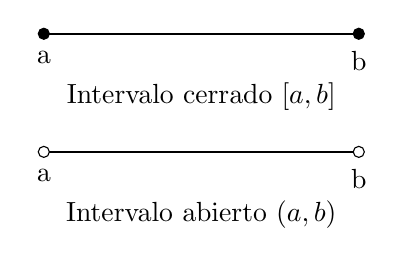
\begin{tikzpicture}
    % Intervalo cerrado
    \draw[thick] (0,0) -- (4,0);
    \filldraw[black] (0,0) circle (2pt);
    \filldraw[black] (4,0) circle (2pt);
    \node[below] at (0,-0.1) {a};
    \node[below] at (4,-0.1) {b};
    \node[below] at (2,-0.5) {Intervalo cerrado $[a, b]$};
    
    % Intervalo abierto
    \draw[thick] (0,-1.5) -- (4,-1.5);
    \draw[fill=white] (0,-1.5) circle (2pt);
    \draw[fill=white] (4,-1.5) circle (2pt);
    \node[below] at (0,-1.6) {a};
    \node[below] at (4,-1.6) {b};
    \node[below] at (2,-2) {Intervalo abierto $(a, b)$};
\end{tikzpicture}
\end{center}

\subsubsection{Desigualdad.}

Una desigualdad es una relación que compara dos expresiones, indicando que una es mayor o menor que la otra. Las desigualdades se pueden clasificar como:

\begin{itemize}
    \item \textbf{Desigualdades estrictas}: Utilizan los símbolos \(<\) (menor que) y \(>\) (mayor que), por ejemplo, \(x < 5\) significa que \(x\) es menor que 5.
    \item \textbf{Desigualdades no estrictas}: Utilizan los símbolos \(\leq\) (menor o igual que) y \(\geq\) (mayor o igual que), por ejemplo, \(x \leq 5\) significa que \(x\) es menor o igual a 5.
\end{itemize}

\subsubsection{Propiedades de la desigualdad.}

Las desigualdades tienen varias propiedades que facilitan su manejo:

\begin{itemize}
    \item \textbf{Transitiva}: Si \(a > b\) y \(b > c\), entonces \(a > c\).
    \item \textbf{Adición y sustracción}: Si \(a > b\), entonces \(a + c > b + c\) y \(a - c > b - c\) para cualquier \(c\).
    \item \textbf{Multiplicación y división}: 
        \begin{itemize}
            \item Si \(a > b\) y \(c > 0\), entonces \(ac > bc\) y \(\frac{a}{c} > \frac{b}{c}\).
            \item Si \(a > b\) y \(c < 0\), entonces \(ac < bc\) y \(\frac{a}{c} < \frac{b}{c}\) (las desigualdades se invierten).
        \end{itemize}
\end{itemize}

\subsection{Operaciones y procedimientos}

\subsubsection{Resolver desigualdades lineales en forma gráfica y analítica.}

Para resolver una desigualdad lineal, podemos usar métodos gráficos y analíticos.

\textbf{Método gráfico}: Consiste en representar la desigualdad en una recta numérica y determinar las regiones que cumplen con la desigualdad. Por ejemplo, para la desigualdad \(x > 3\), se dibuja una línea desde \(x = 3\) hacia la derecha con un círculo abierto en 3.

\textbf{Método analítico}: Involucra manipular algebraicamente la desigualdad para aislar la variable. Aquí hay algunos ejemplos:

\begin{example}
Resolver la desigualdad \(2x - 5 < 3\).

\begin{enumerate}
    \item Sumamos 5 a ambos lados: \(2x < 8\).
    \item Dividimos ambos lados por 2: \(x < 4\).
\end{enumerate}

La solución es \(x < 4\), que se representa en la recta real con un círculo abierto en 4 y una línea que se extiende hacia la izquierda.
\end{example}

\begin{example}
Resolver la desigualdad \(\frac{x - 2}{3} \geq 1\).

\begin{enumerate}
    \item Multiplicamos ambos lados por 3: \(x - 2 \geq 3\).
    \item Sumamos 2 a ambos lados: \(x \geq 5\).
\end{enumerate}

La solución es \(x \geq 5\), que se representa con un círculo cerrado en 5 y una línea hacia la derecha.
\end{example}

\subsection{Aplicaciones}

Las desigualdades lineales se utilizan en diversas aplicaciones, como problemas de optimización y economía. Por ejemplo, determinar la cantidad mínima o máxima de un recurso que se debe utilizar para cumplir con ciertas restricciones.
